\chapter{Installing and launching MeerK40t}
\label{ch:install}

This chapter gets the program onto your computer and onto the screen. Nothing in
it touches the laser.

\section{Three ways to install}

\subsection*{A. Download a ready-made build (recommended for most people)}

Go to the MeerK40t releases page on GitHub and download the file for your
platform. The builds are self-contained: there is nothing else to install, no
Python, no libraries. On Windows it is an installer or a portable executable; on
macOS it is an application bundle; on Linux there are AppImage-style and archive
builds for x86-64 and for the Raspberry~Pi.

\begin{warnbox}[Stable release or weekly build?]
The project publishes two kinds of build. \textbf{Releases} (for example
0.9.9000) are the versions to use when you want the machine to work. \textbf{Weekly
builds} are automated snapshots of the development branch: they contain new
features and new bugs, and they are explicitly not for production work. If you
want the newest feature, expect to test it on scrap.
\end{warnbox}

\subsection*{B. Install with pip}

If you already have Python 3.6 or newer, one command installs the program and
the console entry point:

\begin{lstlisting}[style=konsole]
pip install meerk40t[all]
meerk40t
\end{lstlisting}

\noindent The \cmd{[all]} extra pulls in the GUI (wxPython), image support
(Pillow), camera and tracing support (OpenCV) and DXF import (ezdxf). Without it
you get the headless core: USB, serial and numpy. The individual extras are
\cmd{gui}, \cmd{cam}, \cmd{camhead} and \cmd{dxf}, so
\cmd{pip install meerk40t[gui,dxf]} is a reasonable minimal GUI install.

\subsection*{C. Run from source (for developers and the curious)}

\begin{lstlisting}[style=konsole]
git clone https://github.com/meerk40t/meerk40t.git
cd meerk40t
python -m pip install -r requirements.txt
python meerk40t.py
\end{lstlisting}

\noindent On Linux, three optional system packages add speed and polish. They are
worth installing if your distribution packages them:

\begin{lstlisting}[style=konsole]
# faster bitmap vectorisation (pypotrace)
sudo apt install libagg-dev libpotrace-dev && pip install pypotrace
# faster and better path offsetting, used by kerf compensation (pyclipr)
sudo apt install cmake libeigen3-dev && pip install pyclipr
# only needed if you must build wxPython yourself
sudo apt install libgtk-3-dev libpython3-dev
\end{lstlisting}

\noindent The repository also ships helper scripts: \file{install-run.sh}
(Linux/macOS) and \file{install_run.bat} (Windows) install the requirements, ask
about the optional packages, and start the program.

\begin{notebox}[What you should see afterwards]
Whichever route you chose, you now have either an application to launch from your
desktop, or a \cmd{meerk40t} command in your shell. Running
\cmd{meerk40t --version} prints the name and version, for example
\cmd{MeerK40t 0.9.9040}. The version string has a suffix that tells you how the
program was obtained: \cmd{ pkg} for a packaged install, \cmd{ git} followed by
the branch name when running from a git checkout, and \cmd{ src} when running
from an unpacked source tree.
\end{notebox}

\section{The first launch}

The very first time you start MeerK40t it creates a settings file, shows its main
window, and --- because it does not yet know what hardware you own --- asks you
what kind of machine you have.

\begin{figure}[htbp]
\centering
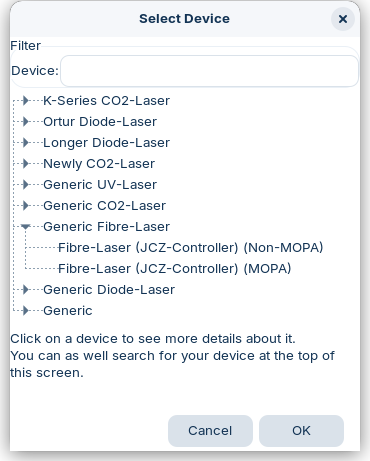
\includegraphics[width=0.62\textwidth]{../screenshots/devices.png}
\caption{The device chooser on a first run. Type a few letters into the
\btn{Device:} filter box to narrow the tree; the list groups generic profiles
(CO\textsubscript{2}, diode, fibre, UV) underneath the drivers that serve them.
Click a device to read its description, then \btn{OK}.}
\label{fig:devices-dialog}
\end{figure}

\noindent Notice the shape of the list. The first level is a family ---
\emph{K-Series CO\textsubscript{2}-Laser}, \emph{Ortur Diode-Laser},
\emph{Longer Diode-Laser}, \emph{Newly CO\textsubscript{2}-Laser}, \emph{Generic
UV-Laser}, \emph{Generic CO\textsubscript{2}-Laser}, \emph{Generic
Fibre-Laser} (with JCZ variants), \emph{Generic Diode-Laser}, and a plain
\emph{Generic} entry. Picking one creates a device that is pre-filled with
sensible defaults for that family; the model name only decides defaults, and every
default can be changed afterwards (Chapter~\ref{ch:connect}).

\begin{behindbox}[What got written to disk]
MeerK40t keeps everything it remembers --- device list, window layout, operation
defaults, recent files, your theme --- in a single text configuration file. It is
written when the program shuts down cleanly, and the previous five versions are
kept as backups beside it.

\begin{center}\small
\begin{tabular}{@{}ll@{}}
\toprule
\textbf{Platform} & \textbf{Location} \\
\midrule
Linux & \file{~/.config/MeerK40t/MeerK40t.cfg} \\
macOS & \file{~/Library/Application Support/MeerK40t/MeerK40t.cfg} \\
Windows & \file{\%LOCALAPPDATA\%\textbackslash MeerK40t\textbackslash MeerK40t.cfg} \\
\bottomrule
\end{tabular}
\end{center}

\noindent Backups are \file{MeerK40t.bak}, \file{MeerK40t.ba1} \dots{}
\file{MeerK40t.ba5}, newest first. When something about the program has gone
strange --- a pane is missing, a device will not connect --- the cure is more
often than not to shut the program down, rename this file aside, and start again.
You will then be asked what device you own, exactly as on a first run.
\end{behindbox}

\section{Starting the program in different ways}

The graphical interface is the default. The same binary is also a scriptable
console program, which is what makes unattended and headless use possible. These
are the command line options:

\begin{center}\small
\begin{tabular}{@{}L{5.4cm}L{8.5cm}@{}}
\toprule
\textbf{Option} & \textbf{Effect} \\
\midrule
\cmd{input} & An input file to open at startup (a positional argument: put the
file name last, or first, but not after a flag that takes a value). \\
\cmd{-o}, \cmd{--output} \cmd{FILE} & An output file name. \\
\cmd{-V}, \cmd{--version} & Print \cmd{MeerK40t <version>} and exit. \\
\cmd{-z}, \cmd{--no-gui} & Run without the graphical interface. \\
\cmd{-Z}, \cmd{--gui-suppress} & Suppress the GUI completely --- never even try
to create a window. Useful on a headless server or over a serial-only
link. \\
\cmd{-w}, \cmd{--simpleui} & Start in the simplified interface
(Chapter~\ref{ch:interface}). \\
\cmd{-c}, \cmd{--console} & Start as a console session: the command prompt is
where you work. \\
\cmd{-e}, \cmd{--execute} \cmd{"CMD"} & Execute a console command, then continue
(or exit, in console mode). May be given more than once. \\
\cmd{-b}, \cmd{--batch} \cmd{FILE} & Run a file of console commands, one per
line. \\
\cmd{-a}, \cmd{--auto} & Start running the laser as soon as the program is
up. \\
\cmd{-q}, \cmd{--quit} & Quit when the spooler has finished --- the batch
combination. \\
\cmd{-d}, \cmd{--daemon} & Keep MeerK40t running in the background after the
job. \\
\cmd{-s}, \cmd{--set} \cmd{key=value} & Set a device or kernel setting at
startup, e.g.\ \cmd{-s bed_width=400mm}. May be repeated. \\
\cmd{-p}, \cmd{--no-plugins} & Do not load external plugins (a plugin
troubleshooting switch). \\
\cmd{-X}, \cmd{--nuke-settings} & Ignore the configuration file at startup ---
effectively a factory-fresh run, without deleting anything. \\
\cmd{-L}, \cmd{--language} \cmd{xx} & Force the interface language: \cmd{en},
\cmd{de}, \cmd{es}, \cmd{fr}, \cmd{hu}, \cmd{it}, \cmd{ja}, \cmd{nl},
\cmd{pt\_BR}, \cmd{pt\_PT}, \cmd{zh}, \cmd{ru}. \\
\cmd{-u}, \cmd{--lock-device-config} & Lock the device configuration so it
cannot be edited (a kiosk / shared-machine switch). \\
\cmd{-U}, \cmd{--lock-general-config} & Lock the general configuration. \\
\cmd{-m}, \cmd{--minimized} & Start with the window minimised. \\
\cmd{-M}, \cmd{--maximized} & Start with the window maximised. \\
\cmd{-A}, \cmd{--disable-ansi} & Disable ANSI colour output in the console. \\
\cmd{-v}, \cmd{--verbose} & Print verbose debugging output. \\
\cmd{-f}, \cmd{--profiler} \cmd{FILE} & Record a Python profile of the session
into a file (for bug reports about speed). \\
\cmd{-P}, \cmd{--profile} \cmd{N} & Accepted but currently unused: the settings
file name is fixed. \\
\bottomrule
\end{tabular}
\end{center}

\noindent A few combinations are worth knowing by heart:

\begin{lstlisting}[style=konsole]
# ordinary use
meerk40t

# open a file straight away
meerk40t ~/designs/tag.svg

# headless: load a file, build the job, run it, quit when done
meerk40t -Z -a -q -e "load /home/me/tag.svg" -e "plan copy-selected preprocess validate blob preopt optimize spool"

# a fresh, factory settings run without touching your real configuration
meerk40t -X

# start the simplified interface
meerk40t -w
\end{lstlisting}

\begin{warnbox}[Wayland]
On Linux, MeerK40t forces the X11 backend (\cmd{GDK\_BACKEND=x11}) because
Wayland does not let an application reposition its own top-level windows, which
the dockable pane system relies on. If you start the program from a terminal you
may therefore see it appear through XWayland. This is intentional.
\end{warnbox}

\section{Keeping it up to date}

Packaged installs and source checkouts are updated differently: for a source
checkout, \cmd{git pull} and restart; for a packaged build, download the new
release. The program also contains an updater component that can check the
project's release feed and tell you when a newer version exists
(Chapter~\ref{ch:prefs}).

\begin{tryit}{Get to the main window, with something recognisable on screen}
\begin{enumerate}[label=\arabic*.,leftmargin=1.4em]
  \item Launch MeerK40t.
  \item If the device chooser appears, pick \emph{Generic CO\textsubscript{2}-Laser}
        or the family that matches your machine and press \btn{OK}. You can change
        this later; nothing is permanent.
  \item Look at the title bar. It reads something like
        \file{MeerK40t v0.9.9040 pkg - lihuyu-device - <file>}: application
        version, active device, and the currently open file.
  \item Find the \panel{Laser-Control} pane and confirm it is not complaining about
        a missing connection. The exact message depends on your driver
        (Chapter~\ref{ch:connect}).
  \item In the \panel{Console} pane, type \cmd{help} and press \key{Enter}. You
        should get a list of commands. This pane is your instrument panel for the
        rest of the manual.
  \item Close the program. Reopen it. The window should come back exactly as you
        left it. That is your settings file working.
\end{enumerate}
\end{tryit}

\noindent If step 6 fails --- if the window comes back scrambled, or a pane is
missing --- you have found the one failure mode worth knowing early. Quit the
program, move \file{MeerK40t.cfg} aside, and start again. You lose your layout,
not your work.
